\documentclass[12pt,a4paper,twoside,openright]{report}
	\usepackage[pdfborder={0 0 0}]{hyperref}    % turns references into hyperlinks
	\usepackage[margin=25mm]{geometry}  % adjusts page layout
	\usepackage{graphicx}  % allows inclusion of PDF, PNG and JPG images
	\usepackage{verbatim}
	\usepackage{docmute}   % only needed to allow inclusion of proposal.tex
	\usepackage{import} %import proposal from another folder
	\usepackage{pdfpages}
	\usepackage{listings}

	\raggedbottom                           % try to avoid widows and orphans
	\sloppy
	\clubpenalty1000%
	\widowpenalty1000%
	
	\renewcommand{\baselinestretch}{1.1}    % adjust line spacing to make
																					% more readable
	
	\begin{document}
	
	\bibliographystyle{plain}
	
	
	%%%%%%%%%%%%%%%%%%%%%%%%%%%%%%%%%%%%%%%%%%%%%%%%%%%%%%%%%%%%%%%%%%%%%%%%
	% Title
	
	
	\pagestyle{empty}
	
	\rightline{\LARGE \textbf{Charlie Crisp}}
	
	\vspace*{60mm}
	\begin{center}
	\Huge
	\textbf{Building a Blockchain Library for OCaml} \\[5mm]
	Computer Science Tripos -- Part II \\[5mm]
	Pembroke College \\[5mm]
	\today  % today's date
	\end{center}
	
	%%%%%%%%%%%%%%%%%%%%%%%%%%%%%%%%%%%%%%%%%%%%%%%%%%%%%%%%%%%%%%%%%%%%%%%%%%%%%%
	% Proforma, table of contents and list of figures
	
	\pagestyle{plain}
	
	\chapter*{Proforma}
	
	{\large
	\begin{tabular}{ll}
	Name:               & \bf Charlie Crisp                       \\
	College:            & \bf Pembroke College                     \\
	Project Title:      & \bf Building a Blockchain Library for OCaml \\
	Examination:        & \bf Computer Science Tripos -- Part II, July 2018  \\
	Word Count:         & \bf ????\footnotemark[1]\\
	Project Originator: & KC Sivaramakrishnan                    \\
	Supervisor:         & KC Sivaramakrishnan                    \\ 
	\end{tabular}
	}
	\footnotetext[1]{This word count was computed
	by \texttt{detex diss.tex | tr -cd '0-9A-Za-z $\tt\backslash$n' | wc -w}
	}
	\stepcounter{footnote}
	
	
	\section*{Original Aims of the Project}
	
	To build a library in OCaml, which can be used as a building block for Blockchain applications. 
	The library should allow participating nodes to own a shared copy of a Blockchain data structure, agreed upon using consensus.
	Nodes should also be able to commit transactions to the blockchain, which should then be visible to other participating nodes. 
	
	
	\section*{Work Completed}
	
	All that has been completed appears in this dissertation.
	
	\section*{Special Difficulties}
	
	None
	 
	\newpage
	\section*{Declaration}
	
	I, Charlie Crisp of Pembroke College, being a candidate for Part II of the Computer
	Science Tripos, hereby declare that this dissertation and the work described in it are my own work,
	unaided except as may be specified below, and that the dissertation
	does not contain material that has already been used to any substantial
	extent for a comparable purpose.
	
	\bigskip
	\leftline{Signed [signature]}
	
	\medskip
	\leftline{Date [date]}
	
	\tableofcontents
	
	\listoffigures
	
	\newpage
	\section*{Acknowledgements}
	
	I would like to thank KC Sivaramakrishnan for being an extremely helpful supervisor throughout the duration of the dissertation, as well as over the past three years.\\
	I would also like to thank Anil Madhavapeddy for allowing me to use his laptop for the duration of the dissertation, and being a very supportive DoS.\\
	Finally I'd like to thank my friends and family for supporting me through my final year.
	
	%%%%%%%%%%%%%%%%%%%%%%%%%%%%%%%%%%%%%%%%%%%%%%%%%%%%%%%%%%%%%%%%%%%%%%%
	% now for the chapters
	
	\pagestyle{headings}
	
	\chapter{Introduction}
	
	%TODO: Put a description of the project in general. Talk about it being a blockchain library, separate from crypto and using a modified verion of consensus protocols.

	\section{The Blockchain}
	
	The blockchain, in its simplest form, is a series of blocks of data, where each block contains the cryptographic hash of the previous block in the chain. This means that the chain can exhibit arbitrary branching. Figure \ref{fig:mainblockchain} is a graphical representation of a typical blockchain data structure.\\
	The significance of blocks containing hashes of previous blocks, is that if a change were to be made to a previous block, it would change the hashes of all subsequent blocks in the chain. This means that once a block is committed to the blockchain, it cannot be modified. \\
	\\
	\begin{figure}
		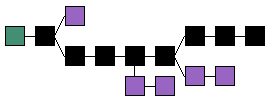
\includegraphics[width=\linewidth]{figs/blockchain}
		\caption{A typical blockchain structure}
		\label{fig:mainblockchain}
	\end{figure}
	
	\section{The History of the Blockchain}
	The blockchain, as a cryptographically secure chain of blocks, was first conceptualised by Stuart Haber and W. Scott Stornetta in 1990 \cite{HaberStornetta}.
	However, until the creation of Git \cite{Git} in 2005, the blockchain was still a relatively niche concept.\\
	Git uses the blockchain as a basis for storing a secure history of code in the form of commits made to branches.
	We will explore the use of the Git as a blockchain during chapter ??? \\
	\\
	The invention of Bitcoin\cite{Bitcoin} in 2008 is seen by many as the most pivotal moment in the history of blockchain technologies.
	Bitcoin combines the blockchain with a 'Proof of Work' consensus algorithm and the result of this is a decentralised, trust-less, peer to peer network which doesn't suffer from the double spending problem. \\
	\\
	\section{Blockchain Today}
	At the time of writing, cryptocurrencies are generating a huge amount of excitement and cynicism in technology and economics communities. The value of Bitcoin is fluctuating on a day-by-day basis and many alternative currencies are gaining in popularity.\\
	For example, Ethereum is a blockchain platform that allows participants to run arbitrary\footnote{Whilst there are restrictions to code run on the blockchain (e.g. it has to be deterministic), the Ethereum language 'Solidity' is Turing complete.} code on the blockchain. These are known as Smart Contracts.

	\chapter{Preparation}
	\section{Starting Point}
		The project will build upon functionality provided by Irmin [1] which is a distributed database system.  Irmin is fast,  durable and has the branching capabilities which are required to build a blockchain.\\
		The project will also make use of Ezirmin \cite{Ezirmin} which provides a simplified API to Irmin.\\
	\section{Using OCaml}
		I had not used OCaml before so I had to learn it. Lwt and all
	\section{Requirements Analysis}
	%TODO: Here I need to put what the technical specification I developed for the project.
	%TODO: Explain the requirement of a blockchain data structure
	%TODO: Explain that there has to be some form of eventual consistency
	%TODO: Explain that it has to tolerate 4+ nodes
	\chapter{Implementation}
	\section{The Blockchain Data Structure}
	\subsection*{Git as a blockchain}
		Git provides a data structure which can be interacted with via a command line API. However, it is not trivial why these data structure is classed as a blockchain. \\
		\\
		In order to convince oneself of this, it is worth considering what features are required for a data structure to be considered a blockchain. 
		Whilst there is no universally agreed definition of a blockchain, it is commonly accepted that it will exhibit the following features:
		\begin{enumerate}
			\item Data is stored in 'blocks'.
			\item Blocks are ordered.
			\item Each block contains a link to its parent block.
		\end{enumerate}
		Now we can consider the promises that Git makes and ensure that the above conditions are satisfied.\\
		\begin{enumerate}
			\item Git stores data as sequences of 'commits' which can be thought of as blocks.
			\item Git history is stored as a tree structure with arbitrary branching. This imposes an order on commits or blocks.
			\item Each Git commit contains the hash of the previous or parent commit.
		\end{enumerate}
		It is clear to see that Git has all the necessary properties to be used as a blockchain data structure.
	\subsection*{Irmin}
		The next question that I needed to answer, was how it was best to interact with an underlying Git protocol, using OCaml. Irmin is a library for OCaml which provides Git-like, distributed, branchable storage \cite{Irmin}.\\
		\\
		Irmin uses a Git backend to store objects which immediately makes it suitable for use as a blockchain. However, it is also possible to consider Irmin's data store at a higher level. \\
		\\
		Irmin provides access to a Block Store and a Tag Store as shown in figure \ref{fig:IrminBlockStore}.
		\begin{figure}
			\begin{center}
			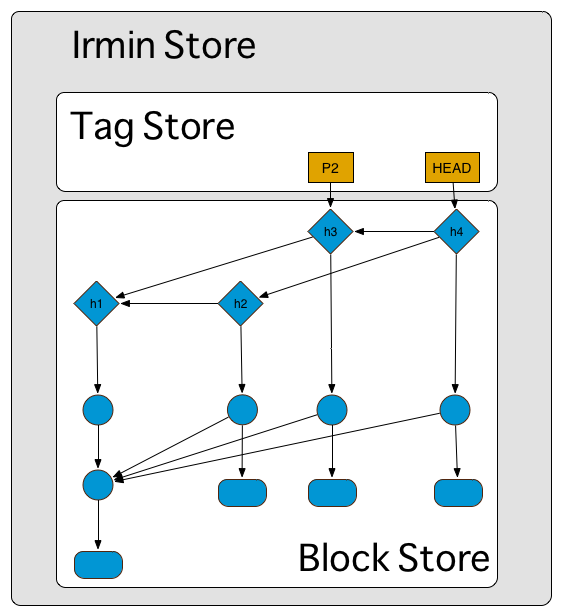
\includegraphics[width=8cm]{figs/irmin-stores.png}
			\caption{Irmin exposes an API for dealing with an mutable tag store and an immutable block store}
			\label{fig:IrminBlockStore}
			\end{center}
		\end{figure}
		The block store is an append-only store of immutable key-value pairs. Mutability comes from the tag store, which provides a way of mapping global branch names to blocks. Both of these stores combine to form an Irmin store with  promises which are beneficial for concurrency. For example, if a tag is not mutated, then you can be sure that the no change in the block store will be visible.\\
		\\
		Irmin Stores can be though of in terms of the following API, expressed in OCaml code. Here, we expose types for keys which address values, and tags which point to keys. The read and update functions allow us to interact with the block store. \\
		\begin{lstlisting}[language=Caml]
  type t
  (* The type for Irmin store. *)

  type tag
  type key 
  type value

  val read: t -> ?branch:tag -> key -> value option
  val update: t -> ?branch:tag -> key -> value -> unit
			
		\end{lstlisting}
		Amongst other different interfaces, Irmin provides a built in API for interacting with an append-only store. This key functionality of this module is expressed in the following code, where \texttt{mem} checks for the presence of a key, \texttt{find} reads values, and \texttt{add} writes to the store.

		\begin{lstlisting}[language=Caml]
  val mem: t -> key -> bool Lwt.t
  val find: t -> key -> value option Lwt.t
  val add: t -> value -> key Lwt.t
		\end{lstlisting}
	\subsection*{Ezirmin}
	Ezirmin is a library that provides a simplified interface to the Irmin library. It is designed to provide a interface to Irmin without functors, but with some useful defaults. Importantly, it has a built in log data structure which uses Irmin's append-only store, saved on disk in the git format.\\
	For this reason, I decided that it would be a suitable data structure to use in this project.
	\section{Mempools}
	When making a transaction using Bitcoin or some other cryptocurrencies, a request for this transaction is placed in what is known as a Mempool\footnote{Mempool is short for Memory Pool}.
	This Mempool can be thought of as a waiting room for transactions. When miners are assembling and mining blocks, this is where they will pick the transactions from.
	
	\section{Consensus Algorithms}
	%TODO: Explain how this was an important part of work.
	%TODO: Explain what are the problems with all of these consensus algorithms and why would they not work in my case.
	%TODO: Explain what the algorithm that I developed is and why it solves these problems
	Typically, cryptocurrencies (which rely on blockchain technology) use a Proof of Work protocol to achieve consensus. 
	There are, however, other ways of achieving consensus, and I evaluated a number of these in order to inform my approach to building consensus into my project. \\ 
		\subsection*{Existing Algorithms}
			\subsubsection*{Proof of Work}
			%TODO: This is good for solving double spending
			%TODO: How does it work in Bitcoin
			%TODO: Use a diagram, mention nonces, yada yada yada
			The proof of work method for achieving consensus is actually very simple. 
			Whenever a block is received by a participating node, the node will check that the block contains a proof of computational work done. 
			In the field of cryptocurrencies, this proof takes the form of a random sequence of data which, when appended to the end of the block, causes its hash to be prefixed with a set number of 0s.
			Because the data appended to the end of a block can only be found by a brute force method, which will require lots of computation/work.
			\subsubsection*{Proof of Stake}
			%TODO: Flesh this out with small amount of detail
			%TODO: Not good for this projects as you need the concept of Stake
			\subsubsection*{Paxos}
			%TODO: Finish
			\subsubsection*{Raft}
			%TODO: Finish description of Raft and it's concept of terms.
		\subsection*{A New Approach}
		%TODO: Overview of my approach to consensus
			\subsection*{Pros and Cons of a Leader Based Approach}
			%TODO: Why is this beneficial? It loosens the trust that comes with a leader based approach.
			%TODO: Might also increase overhead?
			%TODO: Can we do it in a low cost way?
			\subsection*{Writing to the blockchain}
			%TODO: Describe how a participant writes into a mempool that the leader then copies. Participants can then pull from it. 
			\subsection*{How to deal with failure}
			%TODO: If it's a participant then fine. Even if leader changes, that will still be part of the old leaders blockchain.
			%TODO: If it's a leader, then other participants start a leader election.

	\chapter{Evaluation}
	
	\chapter{Conclusion}
	
	
	%%%%%%%%%%%%%%%%%%%%%%%%%%%%%%%%%%%%%%%%%%%%%%%%%%%%%%%%%%%%%%%%%%%%%
	% the bibliography
	\bibliographystyle{plain}
	\bibliography{refs}
	\addcontentsline{toc}{chapter}{Bibliography}
	
	%%%%%%%%%%%%%%%%%%%%%%%%%%%%%%%%%%%%%%%%%%%%%%%%%%%%%%%%%%%%%%%%%%%%%
	% the appendices
	\appendix

	\chapter{Project Proposal}
	
	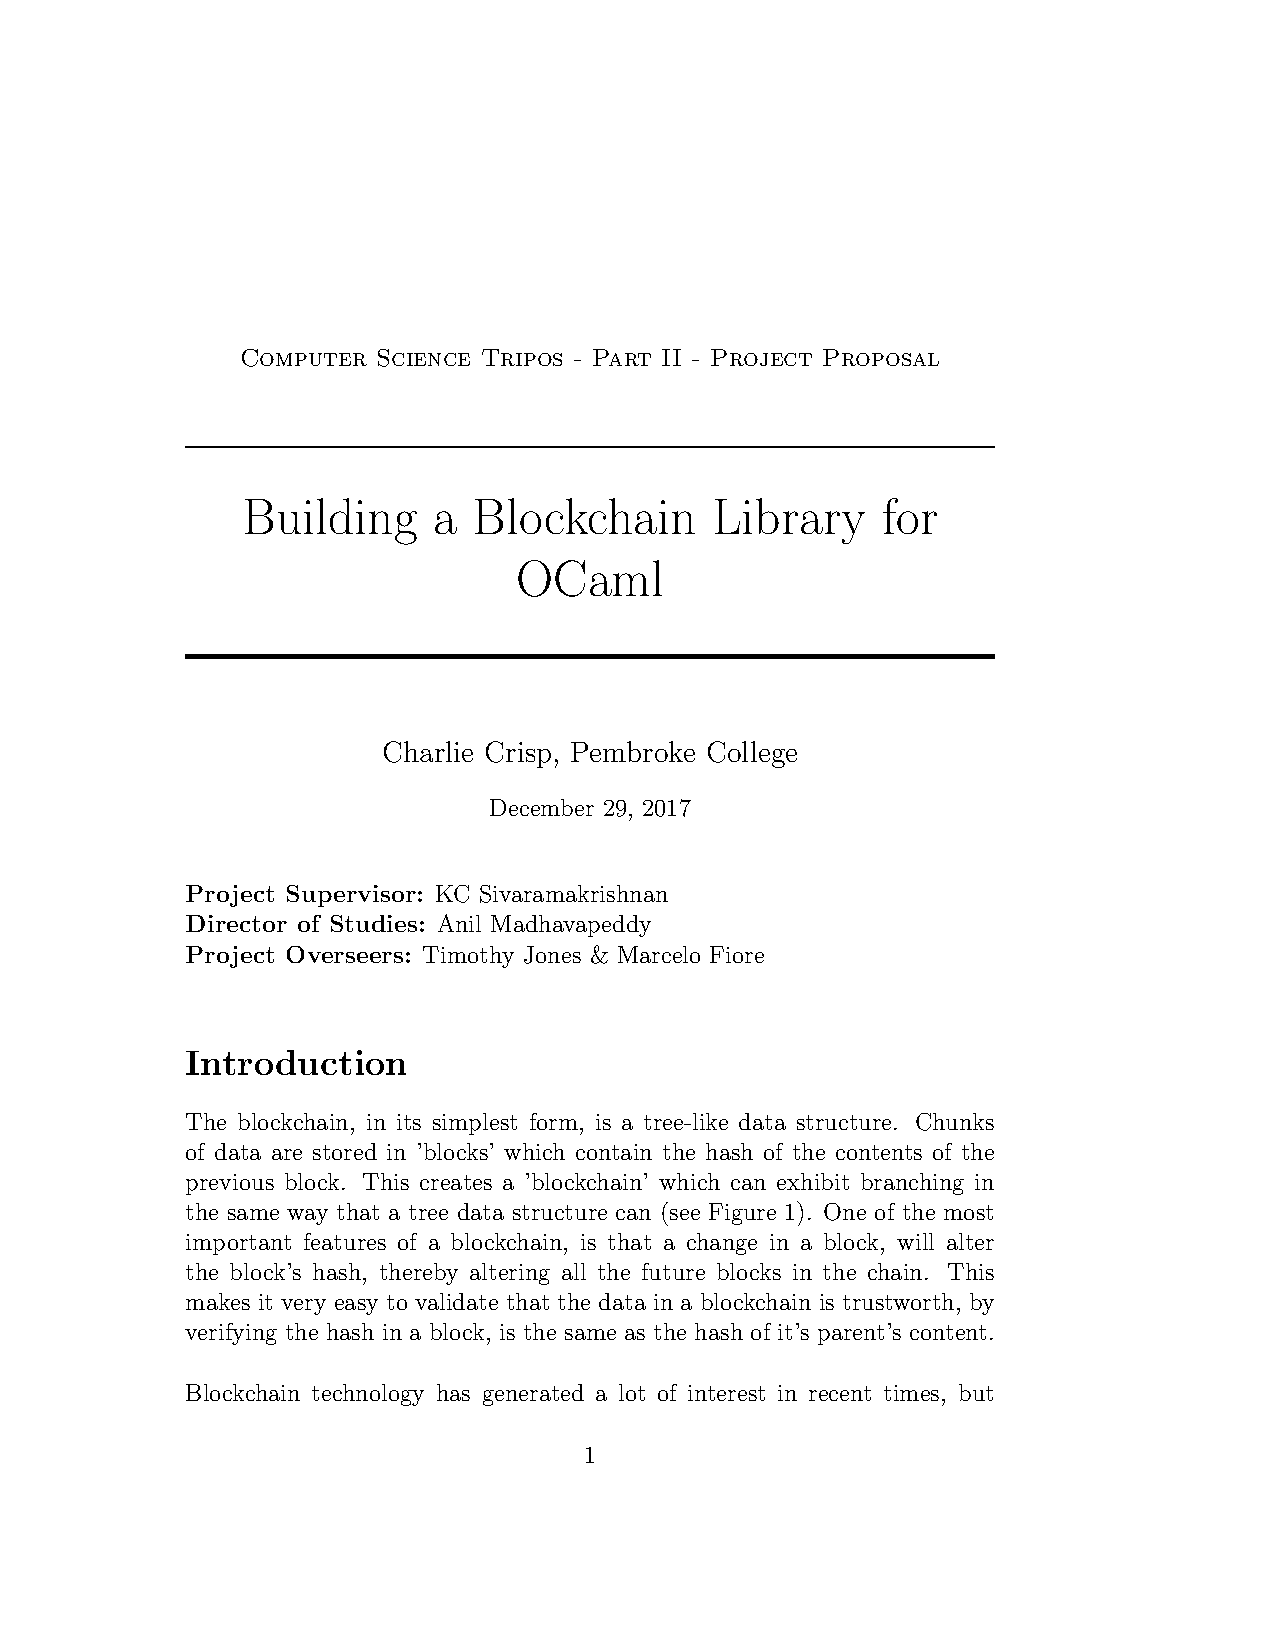
\includepdf[pages=-]{Part_II_Project_Proposal_Draft.pdf}
	
	\end{document}